\section{Preliminaries: The H-SFP Framework}
\label{sec:preliminary}

This section summarizes the conference \hsfp framework that \ehsfp extends.
\hsfp considers a three-tier hierarchy with clients, edge servers, and a cloud server. Let $\clients=\bigcup_{\edgeidx=1}^{M}\clients_{\edgeidx}$ denote the client population, where $\clients_{\edgeidx}$ is the set of clients assigned to edge server $\edgeidx$. A client $k\in\clients_{\edgeidx}$ owns private data $\mathcal{D}_k$ and trains a lightweight client-side encoder. The edge and cloud tiers train the upper model components, so the full model is partitioned across the hierarchy rather than replicated entirely on each client.

\begin{figure}[t]
    \centering
    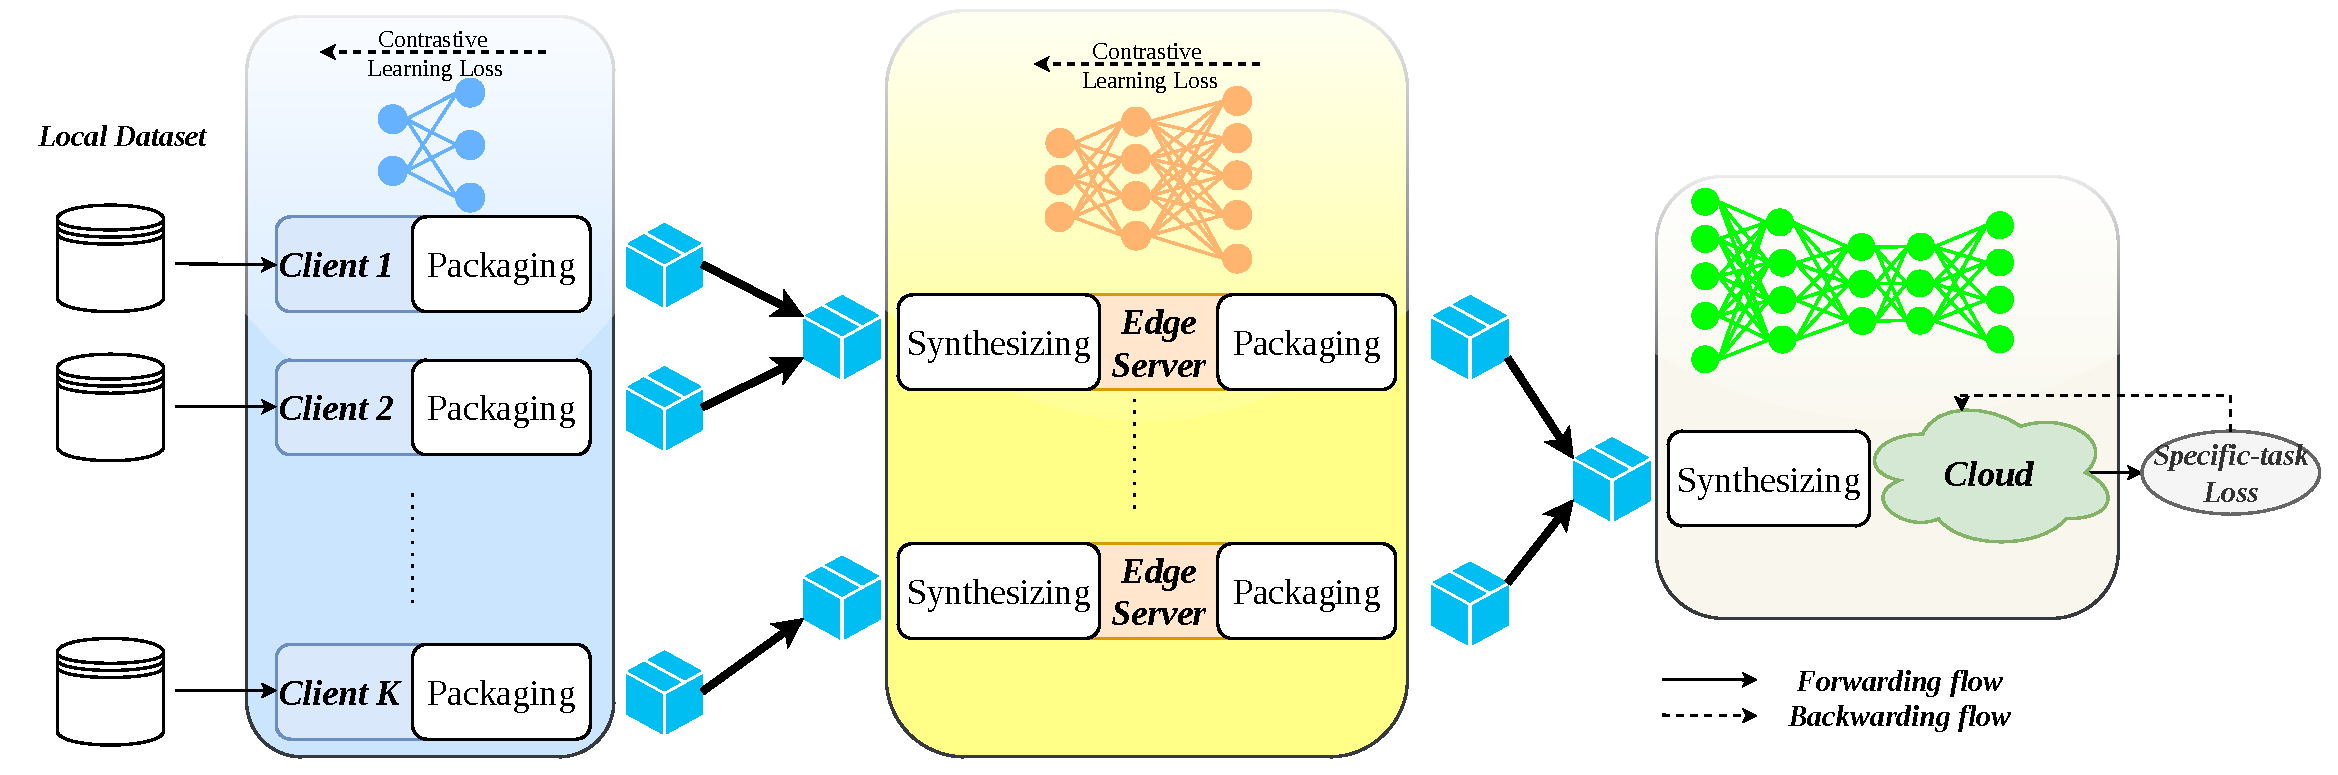
\includegraphics[width=\linewidth]{figures/method-2.pdf}
    \caption{The \hsfp hierarchy. Clients communicate class-wise prototype statistics to edge servers; edge and cloud tiers aggregate statistics, synthesize features, and train their assigned model components without cross-tier backpropagation.}
    \label{fig:hsfp_framework}
\end{figure}

The key design choice in \hsfp is to replace sample-level smashed activations and cross-tier gradients with class-wise prototype statistics. For class $j$, client $k$ computes a feature mean $\pmu_k^{(j)}$, feature standard deviation $\psigma_k^{(j)}$, and support count $n_k^{(j)}$ from its local representation space. The transmitted packet is therefore
\begin{equation}
    P_k^{(j)}=\left(\pmu_k^{(j)},\psigma_k^{(j)},n_k^{(j)}\right),
\end{equation}
rather than a batch of per-sample activations. Edge server $\edgeidx$ aggregates packets from $k\in\clients_{\edgeidx}$ into edge-level class-wise prototype statistics, and the cloud similarly aggregates edge statistics into global class-wise prototype statistics.

Upper tiers then synthesize features from the received statistics. For an aggregated class statistic $(\pmu^{(j)},\psigma^{(j)})$, a synthetic feature is sampled as
\begin{equation}
    z^{(j)} = \pmu^{(j)} + \psigma^{(j)} \odot \epsilon,\qquad
    \epsilon\sim\mathcal{N}(0,I),
    \label{eq:prelim_synthesis}
\end{equation}
which corresponds to a diagonal Gaussian approximation of the lower-tier feature distribution. This Gaussian feature-synthesis strategy follows prior work on prototype-based feature augmentation and exemplar condensation for representation-preserving replay~\cite{9578909,Nguyen_2026_CVPR}. Edge models can train on synthetic client features, and the cloud model can train on synthetic edge features. The lower and upper tiers are therefore optimized through local objectives over their own inputs rather than through one end-to-end backpropagation graph.

\hsfp uses contrastive representation learning at lower tiers, following the NT-Xent contrastive objective ~\cite{chen2020simple}, so that class-wise prototype statistics preserve discriminative structure. The practical benefit is communication reduction: clients send $O(J_k d)$ statistics for $J_k$ observed classes and feature dimension $d$, rather than transmitting activations and gradients for every sample and every split-learning iteration. The methodological limitation, which motivates \ehsfp, is that the original framework assumes comparatively stable prototype availability. It does not explicitly model stateless learning episodes, stale prototype updates, partial prototype updates, missing prototype packets, or asynchronous edge/cloud aggregation.
